\documentclass[10pt]{article}
\usepackage[landscape,letterpaper,margin=0.25in]{geometry}
\usepackage{amsmath,amssymb}
\usepackage[table]{xcolor}
\usepackage{tikz}
\usetikzlibrary{arrows.meta,calc}
\usepackage{booktabs,array}
\pagestyle{empty}
\setlength{\parindent}{0pt}
\setlength{\abovedisplayskip}{2pt}
\setlength{\belowdisplayskip}{2pt}
\setlength{\abovedisplayshortskip}{1pt}
\setlength{\belowdisplayshortskip}{1pt}

\definecolor{cExists}{RGB}{190,235,190}
\definecolor{cNT}{RGB}{255,214,160}
\definecolor{cSub}{RGB}{185,220,245}
\definecolor{cFree}{RGB}{222,222,222}
\definecolor{tExists}{RGB}{20,110,20}
\definecolor{tNT}{RGB}{190,95,0}
\definecolor{tSub}{RGB}{20,80,160}
\definecolor{tFree}{RGB}{95,95,95}
\newcommand{\R}{\mathbb{R}}
\newcommand{\gE}[1]{{\color{tExists}#1}}
\newcommand{\gN}[1]{{\color{tNT}#1}}
\newcommand{\gS}[1]{{\color{tSub}#1}}
\newcommand{\gF}[1]{{\color{tFree}#1}}
\newcommand{\sw}[1]{\tikz[baseline=-0.55ex]\node[draw=black!60,line width=0.3pt,fill=#1,inner sep=2.4pt]{};}

\begin{document}
\begin{minipage}[t]{4.6in}
\vspace{0pt}
{\footnotesize The network $\varphi_\theta:\R^{3\times64\times64}\times\R\to\R^{3\times64\times64}$ used for CelebA at $64\times64$ (channels $\times$ height $\times$ width), $20\,972\,867$ parameters. Each box shows its symbol and parameter count; the space on an arrow is the codomain of the map the arrow leaves. Dashed arrows carry $e=E(t)\in\R^{256}$ into every residual block.}\\[3pt]
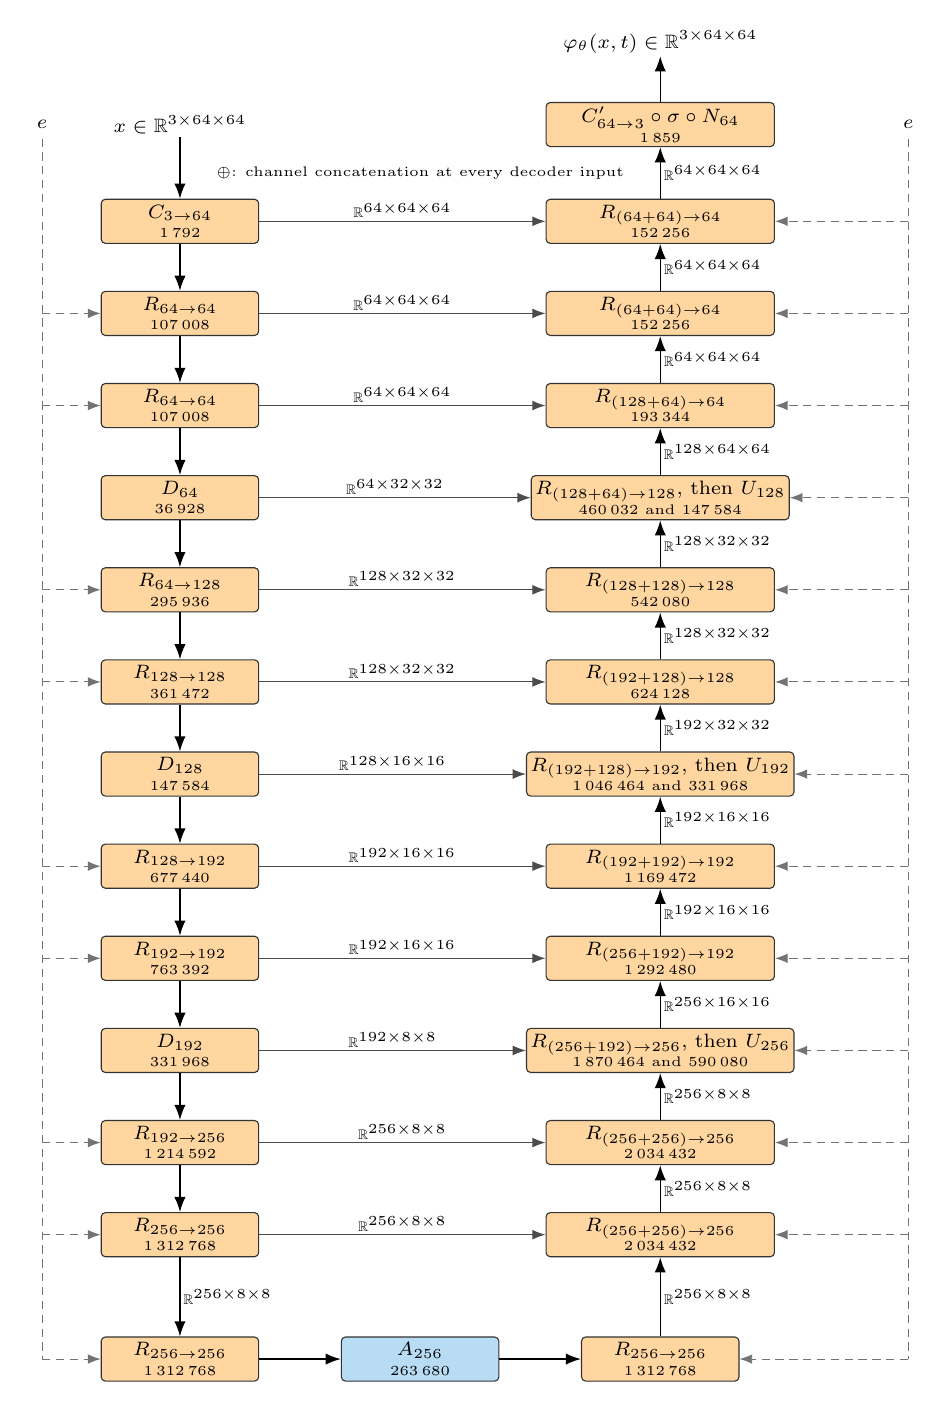
\begin{tikzpicture}[x=1cm,y=-1.17cm,>=Latex,
  blk/.style={draw=black!80,line width=0.4pt,rounded corners=1.5pt,align=center,inner sep=1.4pt,font=\scriptsize,minimum height=0.56cm},
  ebox/.style={blk,minimum width=2.0cm},
  dbox/.style={blk,minimum width=2.9cm},
  nt/.style={fill=cNT},ex/.style={fill=cExists},sb/.style={fill=cSub},fr/.style={fill=cFree},
  flow/.style={->,line width=0.55pt},
  skip/.style={->,line width=0.4pt,draw=black!70},
  ebus/.style={densely dashed,line width=0.35pt,draw=black!55},
  lab/.style={font=\tiny,inner sep=1pt}]
\def\xE{1.2}\def\xD{7.3}
\coordinate (busL) at (-0.55,0);
\coordinate (busR) at (10.45,0);
% encoder column
\node[ebox,nt] (E0) at (\xE,0) {$C_{3\to64}$\\[-1pt]{\tiny $1\,792$}};
\node[ebox,nt] (E1) at (\xE,1) {$R_{64\to64}$\\[-1pt]{\tiny $107\,008$}};
\node[ebox,nt] (E2) at (\xE,2) {$R_{64\to64}$\\[-1pt]{\tiny $107\,008$}};
\node[ebox,nt] (E3) at (\xE,3) {$D_{64}$\\[-1pt]{\tiny $36\,928$}};
\node[ebox,nt] (E4) at (\xE,4) {$R_{64\to128}$\\[-1pt]{\tiny $295\,936$}};
\node[ebox,nt] (E5) at (\xE,5) {$R_{128\to128}$\\[-1pt]{\tiny $361\,472$}};
\node[ebox,nt] (E6) at (\xE,6) {$D_{128}$\\[-1pt]{\tiny $147\,584$}};
\node[ebox,nt] (E7) at (\xE,7) {$R_{128\to192}$\\[-1pt]{\tiny $677\,440$}};
\node[ebox,nt] (E8) at (\xE,8) {$R_{192\to192}$\\[-1pt]{\tiny $763\,392$}};
\node[ebox,nt] (E9) at (\xE,9) {$D_{192}$\\[-1pt]{\tiny $331\,968$}};
\node[ebox,nt] (E10) at (\xE,10) {$R_{192\to256}$\\[-1pt]{\tiny $1\,214\,592$}};
\node[ebox,nt] (E11) at (\xE,11) {$R_{256\to256}$\\[-1pt]{\tiny $1\,312\,768$}};
% middle row
\node[ebox,nt] (M1) at (\xE,12.35) {$R_{256\to256}$\\[-1pt]{\tiny $1\,312\,768$}};
\node[ebox,sb] (M2) at (4.25,12.35) {$A_{256}$\\[-1pt]{\tiny $263\,680$}};
\node[ebox,nt] (M3) at (\xD,12.35) {$R_{256\to256}$\\[-1pt]{\tiny $1\,312\,768$}};
% decoder column (D_j at row 11-j)
\node[dbox,nt] (D0) at (\xD,11) {$R_{(256+256)\to256}$\\[-1pt]{\tiny $2\,034\,432$}};
\node[dbox,nt] (D1) at (\xD,10) {$R_{(256+256)\to256}$\\[-1pt]{\tiny $2\,034\,432$}};
\node[dbox,nt] (D2) at (\xD,9) {$R_{(256+192)\to256}$, then $U_{256}$\\[-1pt]{\tiny $1\,870\,464$ and $590\,080$}};
\node[dbox,nt] (D3) at (\xD,8) {$R_{(256+192)\to192}$\\[-1pt]{\tiny $1\,292\,480$}};
\node[dbox,nt] (D4) at (\xD,7) {$R_{(192+192)\to192}$\\[-1pt]{\tiny $1\,169\,472$}};
\node[dbox,nt] (D5) at (\xD,6) {$R_{(192+128)\to192}$, then $U_{192}$\\[-1pt]{\tiny $1\,046\,464$ and $331\,968$}};
\node[dbox,nt] (D6) at (\xD,5) {$R_{(192+128)\to128}$\\[-1pt]{\tiny $624\,128$}};
\node[dbox,nt] (D7) at (\xD,4) {$R_{(128+128)\to128}$\\[-1pt]{\tiny $542\,080$}};
\node[dbox,nt] (D8) at (\xD,3) {$R_{(128+64)\to128}$, then $U_{128}$\\[-1pt]{\tiny $460\,032$ and $147\,584$}};
\node[dbox,nt] (D9) at (\xD,2) {$R_{(128+64)\to64}$\\[-1pt]{\tiny $193\,344$}};
\node[dbox,nt] (D10) at (\xD,1) {$R_{(64+64)\to64}$\\[-1pt]{\tiny $152\,256$}};
\node[dbox,nt] (D11) at (\xD,0) {$R_{(64+64)\to64}$\\[-1pt]{\tiny $152\,256$}};
\node[dbox,nt] (H) at (\xD,-1.05) {$C'_{64\to3}\circ\sigma\circ N_{64}$\\[-1pt]{\tiny $1\,859$}};
% input / output
\node[lab,font=\scriptsize] (xin) at (\xE,-1.05) {$x\in\R^{3\times64\times64}$};
\node[lab,font=\scriptsize] (yout) at (\xD,-1.95) {$\varphi_\theta(x,t)\in\R^{3\times64\times64}$};
\draw[flow] (xin) -- (E0);
\draw[flow] (H) -- (yout);
% encoder flow
\foreach \i/\j in {0/1,1/2,2/3,3/4,4/5,5/6,6/7,7/8,8/9,9/10,10/11} \draw[flow] (E\i) -- (E\j);
\draw[flow] (E11) -- (M1) node[lab,right,midway] {$\R^{256\times8\times8}$};
\draw[flow] (M1) -- (M2);
\draw[flow] (M2) -- (M3);
\draw[flow] (M3) -- (D0) node[lab,right,midway] {$\R^{256\times8\times8}$};
% decoder flow with codomains
\draw[flow] (D0) -- (D1) node[lab,right,midway] {$\R^{256\times8\times8}$};
\draw[flow] (D1) -- (D2) node[lab,right,midway] {$\R^{256\times8\times8}$};
\draw[flow] (D2) -- (D3) node[lab,right,midway] {$\R^{256\times16\times16}$};
\draw[flow] (D3) -- (D4) node[lab,right,midway] {$\R^{192\times16\times16}$};
\draw[flow] (D4) -- (D5) node[lab,right,midway] {$\R^{192\times16\times16}$};
\draw[flow] (D5) -- (D6) node[lab,right,midway] {$\R^{192\times32\times32}$};
\draw[flow] (D6) -- (D7) node[lab,right,midway] {$\R^{128\times32\times32}$};
\draw[flow] (D7) -- (D8) node[lab,right,midway] {$\R^{128\times32\times32}$};
\draw[flow] (D8) -- (D9) node[lab,right,midway] {$\R^{128\times64\times64}$};
\draw[flow] (D9) -- (D10) node[lab,right,midway] {$\R^{64\times64\times64}$};
\draw[flow] (D10) -- (D11) node[lab,right,midway] {$\R^{64\times64\times64}$};
\draw[flow] (D11) -- (H) node[lab,right,midway] {$\R^{64\times64\times64}$};
% skip connections: E_i -> D_{11-i}, labelled with the encoder codomain
\draw[skip] (E0.east) -- (D11.west) node[lab,above,midway] {$\R^{64\times64\times64}$};
\draw[skip] (E1.east) -- (D10.west) node[lab,above,midway] {$\R^{64\times64\times64}$};
\draw[skip] (E2.east) -- (D9.west) node[lab,above,midway] {$\R^{64\times64\times64}$};
\draw[skip] (E3.east) -- (D8.west) node[lab,above,midway] {$\R^{64\times32\times32}$};
\draw[skip] (E4.east) -- (D7.west) node[lab,above,midway] {$\R^{128\times32\times32}$};
\draw[skip] (E5.east) -- (D6.west) node[lab,above,midway] {$\R^{128\times32\times32}$};
\draw[skip] (E6.east) -- (D5.west) node[lab,above,midway] {$\R^{128\times16\times16}$};
\draw[skip] (E7.east) -- (D4.west) node[lab,above,midway] {$\R^{192\times16\times16}$};
\draw[skip] (E8.east) -- (D3.west) node[lab,above,midway] {$\R^{192\times16\times16}$};
\draw[skip] (E9.east) -- (D2.west) node[lab,above,midway] {$\R^{192\times8\times8}$};
\draw[skip] (E10.east) -- (D1.west) node[lab,above,midway] {$\R^{256\times8\times8}$};
\draw[skip] (E11.east) -- (D0.west) node[lab,above,midway] {$\R^{256\times8\times8}$};
\node[lab] at (4.25,-0.52) {$\oplus$: channel concatenation at every decoder input};
% e buses
\node[font=\scriptsize] (eL) at (-0.55,-1.05) {$e$};
\node[font=\scriptsize] (eR) at (10.45,-1.05) {$e$};
\draw[ebus] (eL.south) -- (busL |- M1.west);
\draw[ebus] (eR.south) -- (busR |- M3.east);
\foreach \n in {E1,E2,E4,E5,E7,E8,E10,E11,M1} \draw[ebus,->] (\n.west -| busL) -- (\n.west);
\foreach \n in {D0,D1,D2,D3,D4,D5,D6,D7,D8,D9,D10,D11,M3} \draw[ebus,->] (\n.east -| busR) -- (\n.east);
\end{tikzpicture}
\end{minipage}\hfill
\begin{minipage}[t]{5.55in}
\vspace{0pt}
\scriptsize
\setlength{\abovedisplayskip}{3pt}\setlength{\belowdisplayskip}{3pt}\setlength{\abovedisplayshortskip}{2pt}\setlength{\belowdisplayshortskip}{2pt}
\textsc{Time conditioning.}\quad
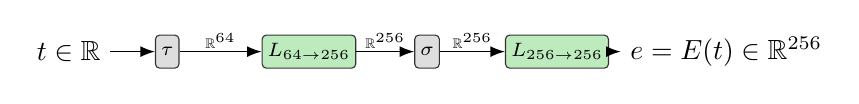
\begin{tikzpicture}[baseline=(t.base),x=1cm,>=Latex,
  blk/.style={draw=black!80,line width=0.4pt,rounded corners=1.5pt,align=center,inner sep=2pt,font=\scriptsize,minimum height=0.42cm},
  flow/.style={->,line width=0.5pt},lab/.style={font=\tiny,inner sep=1pt}]
\node (t) at (0,0) {$t\in\R$};
\node[blk,fill=cFree] (tau) at (1.25,0) {$\tau$};
\node[blk,fill=cExists] (L1) at (3.05,0) {$L_{64\to256}$};
\node[blk,fill=cFree] (s) at (4.55,0) {$\sigma$};
\node[blk,fill=cExists] (L2) at (6.2,0) {$L_{256\to256}$};
\node (e) at (8.35,0) {$e=E(t)\in\R^{256}$};
\draw[flow] (t) -- (tau);
\draw[flow] (tau) -- (L1) node[lab,above,midway] {$\R^{64}$};
\draw[flow] (L1) -- (s) node[lab,above,midway] {$\R^{256}$};
\draw[flow] (s) -- (L2) node[lab,above,midway] {$\R^{256}$};
\draw[flow] (L2) -- (e);
\end{tikzpicture}\\[0pt]
$\gF{\tau}(t)=(\cos\omega_i t)_{i=0}^{31}\oplus(\sin\omega_i t)_{i=0}^{31}\in\R^{64}$, $\omega_i=10^{-4i/32}$; $E$ has $82\,432$ parameters. $\tau$ is the sinusoidal positional table of a transformer evaluated at the real argument $t$ instead of an integer position (same frequencies, same cosine and sine halves).

\vspace{1pt}
\textsc{Residual block} $R_{a\to b}:\R^{a\times h\times w}\times\R^{256}\to\R^{b\times h\times w}$:
\[
R_{a\to b}(z,e)=S(z)+\gN{C'_{b\to b}}\Big(\gF{\sigma}\big(\gS{N_b}\big(\gN{C_{a\to b}}(\gF{\sigma}(\gS{N_a}(z)))\big)\odot(1+s(e))+u(e)\big)\Big),\qquad
[s(e);u(e)]=\gE{L_{256\to2b}}(\gF{\sigma}(e))\in\R^{2b},
\]
with $S=\mathrm{id}$ if $a=b$ and $S=\gE{C^1_{a\to b}}$ otherwise; $s(e),u(e)\in\R^{b}$ scale and shift channels, broadcast over pixels; $C'$ is zero at initialisation (dropout rate $0$). Parameters: $2a+9ab+9b^2+518b+[a\neq b]\,(ab+b)$.

\vspace{1pt}
\textsc{Attention block} $A_a:\R^{a\times h\times w}\to\R^{a\times h\times w}$, used once with $a=256$ on $m=hw=64$ tokens: $z$ is reshaped to $X\in\R^{a\times m}$ and
\[
[Q;K;V]=\gE{W_{qkv}}\,\gS{N_a}(X)+\gE{b_{qkv}},\qquad
H_j=V_j\,\operatorname{softmax}\!\Big(\tfrac{K_j^{\top}Q_j}{\sqrt{a/4}}\Big),\qquad
A_a(X)=X+\gE{W_o}\,[H_1;\dots;H_4]+\gE{b_o},
\]
where $Q_j,K_j,V_j\in\R^{a/4\times m}$ are the rows of head $j=1,\dots,4$, the softmax runs over the key index, $W_{qkv}\in\R^{3a\times a}$, $W_o\in\R^{a\times a}$ (zero at initialisation). Parameters: $4a^2+6a$.

\vspace{1pt}
\textsc{Components.}\\[1pt]
{\tiny
\setlength{\tabcolsep}{2pt}\renewcommand{\arraystretch}{1.0}
\begin{tabular}{@{}>{$}l<{$} >{\raggedright\arraybackslash}p{4.55cm} >{\raggedright\arraybackslash}p{3.9cm} >{$}l<{$} c@{}}
\toprule
\text{symbol} & definition & domain $\to$ codomain & \text{parameters} & \\
\midrule
\tau & sinusoidal embedding (above) & $\R\to\R^{64}$ & 0 & \cellcolor{cFree}\\
L_{a\to b} & $x\mapsto Wx+b$ & $\R^{a}\to\R^{b}$; $(a,b)\in\{(64,256),(256,256)\}$ in $E$ and $(256,2b)$ inside every $R_{\cdot\to b}$ & ab+b & \cellcolor{cExists}\\
\sigma & $x\mapsto x/(1+e^{-x})$ entrywise & $\R^{n}\to\R^{n}$ & 0 & \cellcolor{cFree}\\
N_a & group normalisation: $(z-\mu_g)/\sqrt{v_g+\varepsilon}$ over 32 groups $g$ of $a/32$ channels (statistics over the group's channels and all pixels), then per-channel $\gamma_c z+\beta_c$ & $\R^{a\times h\times w}\to\R^{a\times h\times w}$ & 2a & \cellcolor{cSub}\\
C_{a\to b} & $3\times3$ convolution, stride 1, unit zero padding ($C'$: zero at initialisation) & $\R^{a\times h\times w}\to\R^{b\times h\times w}$ & 9ab+b & \cellcolor{cNT}\\
C^{1}_{a\to b} & $1\times1$ convolution, i.e. $L_{a\to b}$ applied at every pixel & $\R^{a\times h\times w}\to\R^{b\times h\times w}$ & ab+b & \cellcolor{cExists}\\
D_a & $3\times3$ convolution, stride 2, unit zero padding & $\R^{a\times h\times w}\to\R^{a\times h/2\times w/2}$ & 9a^2+a & \cellcolor{cNT}\\
U_a & nearest-neighbour upsampling by 2 (parameter-free), then $C_{a\to a}$ & $\R^{a\times h\times w}\to\R^{a\times 2h\times 2w}$ & 9a^2+a & \cellcolor{cNT}\\
\oplus & channel concatenation (every decoder input) & $\R^{a\times h\times w}\times\R^{b\times h\times w}\to\R^{(a+b)\times h\times w}$ & 0 & \cellcolor{cFree}\\
R_{a\to b} & residual block (formula above) & $\R^{a\times h\times w}\times\R^{256}\to\R^{b\times h\times w}$ & \text{see above} & \cellcolor{cNT}\\
A_a & attention block (formula above) & $\R^{a\times h\times w}\to\R^{a\times h\times w}$ & 4a^2+6a & \cellcolor{cSub}\\
\text{head} & $C'_{64\to3}\circ\sigma\circ N_{64}$ & $\R^{64\times64\times64}\to\R^{3\times64\times64}$ & 1\,859 & \cellcolor{cNT}\\
\bottomrule
\end{tabular}}

\vspace{1pt}
\textsc{Colour legend.}\quad
\sw{cExists} exists as an object of the sparse-transformers classes: an affine map applied per token or per pixel is a sparse linear layer with fan-in $K$ ($K=n_{\mathrm{in}}$ is the dense layer): the time path, the scale-shift maps, the $1\times1$ convolutions, the attention projections.\quad
\sw{cNT} could reasonably be made sparse but is not one of those objects: a $3\times3$ convolution is a parameter-free unfold (gather of the $3\times3\times a$ neighbourhood of a pixel) followed by a per-pixel linear map $\R^{9a}\to\R^{b}$, a sparse linear layer with $K\le9a$, but with weights shared across pixels and a structured, not random, support.\quad
\sw{cSub} could be substituted: softmax attention by attention-free attention or windowed causal attention (both causal), group normalisation by dynamic-tanh or root-mean-square normalisation.\quad
\sw{cFree} parameter-free.\quad
A composite box ($R$, $D$, $U$, head) takes the colour of its weight-carrying parts; its formula colours each factor.

\vspace{1pt}
\textsc{Fan-in.}\quad A sparse linear layer $S:\R^{n_{\mathrm{in}}}\to\R^{n_{\mathrm{out}}}$ with fan-in $K$ computes $S(x)=(M\odot W)\,x+b$ with $M\in\{0,1\}^{n_{\mathrm{out}}\times n_{\mathrm{in}}}$, $\sum_{j}M_{ij}=K$ for every $i$, the $K$ nonzero entries of each row drawn uniformly without replacement, $W\in\R^{n_{\mathrm{out}}\times n_{\mathrm{in}}}$ trained and $\odot$ entrywise; $K$ is clamped to $1\le K\le n_{\mathrm{in}}$ and $K=n_{\mathrm{in}}$ gives the dense map $L$ (the masked dense weight and the $n_{\mathrm{out}}\times K$ weight with an index table are two implementations of the same map). In the graph whose edges are the pairs $(i,j)$ with $M_{ij}=1$ the constraint fixes in-degrees only:
\[
k^{-}_i=\sum_j M_{ij}=K\ \text{(output unit } i),\qquad d^{+}_j=\sum_i M_{ij}\ \text{(input unit } j),\qquad \mathbb{E}\,d^{+}_j=\frac{n_{\mathrm{out}}K}{n_{\mathrm{in}}}.
\]
In a stack of layers $l=1,\dots,L$ with widths $n_0,\dots,n_L$ and fan-ins $K_l$, a hidden unit $v$ of layer $l$ ($0<l<L$) has degree $k_v=K_l+d^{+}_v$, so the maximum degree of the network graph obeys
\[
K_G:=\max_v k_v\ \ge\ \max_l K_l,\qquad \mathbb{E}\,k_v=K_l+\frac{n_{l+1}K_{l+1}}{n_l},
\]
with equality only in the degenerate case where every hidden unit of layer $l$ has out-degree at most $\max_{l'}K_{l'}-K_l$, which the random supports do not enforce. The fan-in $K$ (per layer, $K_l$) is therefore the quantity of interest, not $K_G$; a green box is a map of the form $S$ with any $K\le n_{\mathrm{in}}$.
\end{minipage}
\end{document}
